\documentclass[12pt]{article}
\usepackage{titlesec}
\usepackage{subcaption}
\usepackage[scaled]{helvet}  \renewcommand\familydefault{\sfdefault} % Font
\usepackage{graphicx} % Required for inserting images
\usepackage{geometry}
\usepackage[colorlinks=true, urlcolor=blue, linkcolor=red]{hyperref}
\usepackage{pgfplotstable}
\usepackage{amsmath}
\usepackage{enumitem}
\usepackage{tikz} 
\usetikzlibrary{petri,arrows.meta}
\geometry{a4paper, total={170mm,257mm},left=20mm, top=20mm,}
\usepackage[listings,breakable,skins]{tcolorbox}
% declare our code block environment
  \newtcblisting{tcbcodeblock}[1]{%
    enhanced,
    sharp corners,
    colframe=black,
    coltext=codefg,
    colback=codebg,
    breakable,
    size=fbox,
    listing only,
    listing options={%
      style=tcblatex,
      language={#1},
      showspaces=false,
      showstringspaces=false,
      commentstyle=\color{codegray},
      keywordstyle=\color{codegreen},
      stringstyle=\color{codecyan},
      basicstyle=\ttfamily\footnotesize
    }
  }
\renewcommand{\thesection}{\Roman{section}}
\renewcommand{\thesubsection}{\arabic{subsection}}
\renewcommand{\thesubsubsection}{\alph{subsubsection}.}

\titleformat{\section}{\normalfont\LARGE\bfseries}{\thesection.}{10pt}{}
\titleformat{\subsection}{\normalfont\Large}{\thesubsection.}{10pt}{}
\titleformat{\subsubsection}{\normalfont\large}{\thesubsubsection}{10pt}{}

\begin{document}
\thispagestyle{empty} %Suppress number of this page
\begin{center}
    \vspace{7pt}
    \fontsize{18pt}{17pt}\selectfont 
    \textbf{University of Science and Technology of Hanoi}
    \vspace{7pt}
\end{center}
\vspace{10pt}
\begin{center}
    
\includegraphics[scale=0.4]{USTH.png}
\end{center}

\vspace{90pt}

\begin{center}
    \fontsize{30pt}{17pt}\selectfont 
    \textbf{Subject} 
    \vspace{50pt}

    \fontsize{20pt}{17pt}\selectfont 
    \textbf{Advanced programming HPC Labwork 2}
    \vspace{50pt}


    \fontsize{17pt}{17pt}\selectfont
    \textbf{{Student id: }{ict2440050}}
    \vspace{15pt}

    \fontsize{17pt}{17pt}\selectfont
    \textbf{{Student name: }{Nguyen Vu Bach}}
    \vspace{15pt}
    
\end{center}

\newpage
\setcounter{page}{1} % Start number from this page
\section{Device}
\begin{figure}[h!]
    \centering
    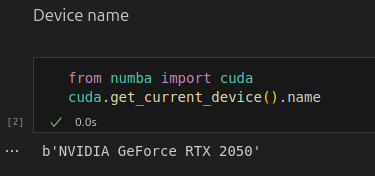
\includegraphics[width=0.5\linewidth]{DeviceInfo.png}
    \caption{Device name}
    \label{fig:placeholder}
\end{figure}

I use \(\textbf{get\_current\_device}\) to get the device name which is 'NVIDIA GeForce RTX 2050'

\section{Core}
\begin{figure}[h!]
    \centering
    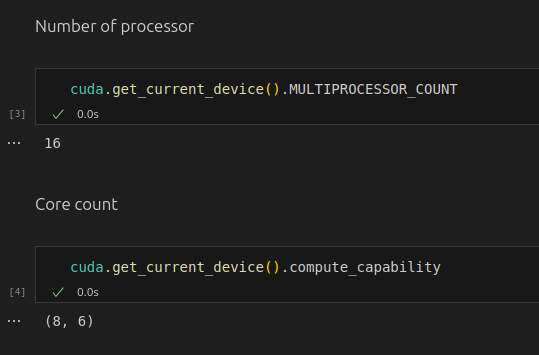
\includegraphics[width=0.5\linewidth]{CoreInfo.png}
    \caption{Core info}
    \label{fig:placeholder}
\end{figure}
I use \(\textbf{get\_current\_device().MULTIPROCESSOR\_COUNT}\) to get the RTX 2050 number of multiprocessor and compute capabilities which is 16 and (8,6). the compute capabilitie is a versioning system used by NVIDIA to describe the feature set of their GPUs.


\newpage
\begin{figure}[h!]
    \centering
    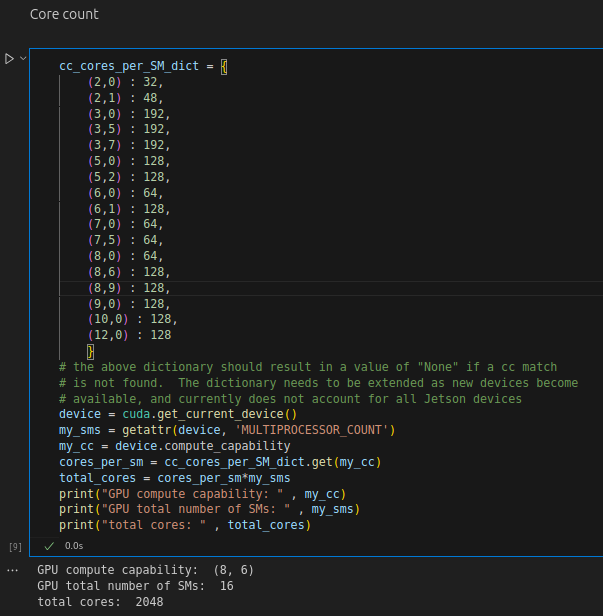
\includegraphics[width=0.5\linewidth]{CoreCount.png}
    \caption{Core count}
    \label{fig:placeholder}
\end{figure}

I copied the code from \href{https://stackoverflow.com/questions/63823395/how-can-i-get-the-number-of-cuda-cores-in-my-gpu-using-python-and-numba}{Stackoverflow} to get the number of cores.
% \subsection{Subsection}

\section{Memory}
\begin{figure}[h!]
    \centering
    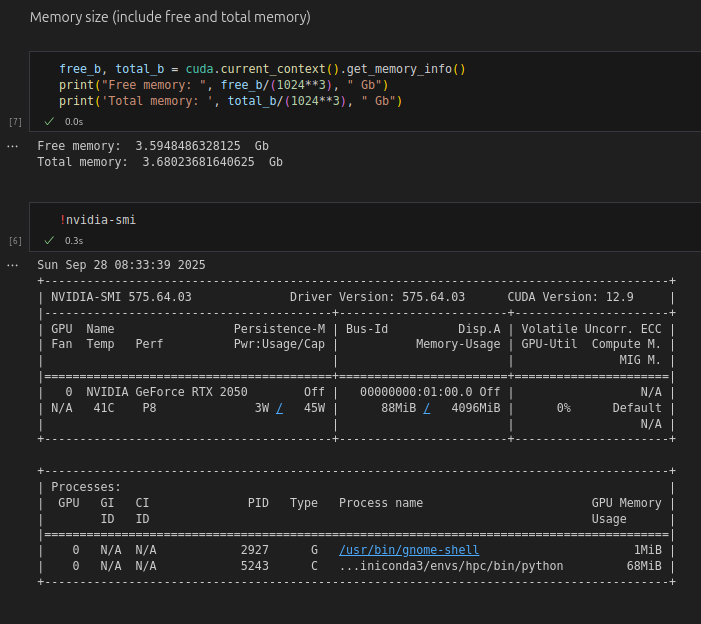
\includegraphics[width=0.5\linewidth]{Memory.png}
    \caption{Memory Info}
    \label{fig:placeholder}
\end{figure}

\(\textbf{current\_context().get\_memory\_info()}\) is used to get free and total memory of device. But when I run \(\textbf(!nvidia-smi)\), it show that I have 4Gb of memory instead of 3.6Gb. This means last 0,4Gb is not occupied for computation.


\end{document}







